\documentclass{article}
\usepackage[utf8]{inputenc}
\usepackage[english]{babel}
\usepackage{multicol}
\usepackage[a4paper, total={8in, 10in}]{geometry}
\usepackage{graphicx}
\usepackage{color}
\usepackage{listings}
\usepackage{listings-golang} % import this package after listings
\usepackage{amsfonts} 

\title{Fonálinga periódusideje nagy szögekre}
\author{Vörös Asztrik}
\date{}
\definecolor{brown}{RGB}{178,141,103}
\definecolor{green-dark}{RGB}{94,153,85}
\lstset{
    language=Go,
	basicstyle=\ttfamily\footnotesize,
    numberstyle=\footnotesize,
    numbers=left,
    frame=single,
    tabsize=2,
    breaklines=true,
    breakatwhitespace=true,
    framextopmargin=2pt,
    framexbottommargin=2pt,
    inputencoding=utf8,
	extendedchars=true,
	showstringspaces=false,
	literate=
		{ü}{{\"{u}}}1
		{ű}{{\H{u}}}1
		{ö}{{\"{o}}}1
		{é}{{\'{e}}}1
		{í}{{\'{i}}}1
		{á}{{\'{a}}}1
		{∈}{{$\in$}}1
		{π}{{$\pi$}}1
		{√}{{$\sqrt{}$}}1,
	keywordstyle=\color{blue}\ttfamily,
	stringstyle=\color{brown}\ttfamily,
	commentstyle=\color{green-dark}\ttfamily,
}

\begin{document}
\maketitle

\abstract{
	A modellezés célja, hogy megállapítsuk egy adott hosszúságú
	inga periódusidejét nagy szögekre is, majd a százalékos
	eltérést kimutassuk a kis szögekre adott képlethez képest.
	A metódust felhasználva szintén meghatározhatjuk, hogy adott
	hibahatáron belül maradáshoz maximum mekkora szöggel
	téríthetjük ki az ingát.
}

\begin{multicols}{2}

\section{Dinamikai jellemzés}
	\begin{center}
		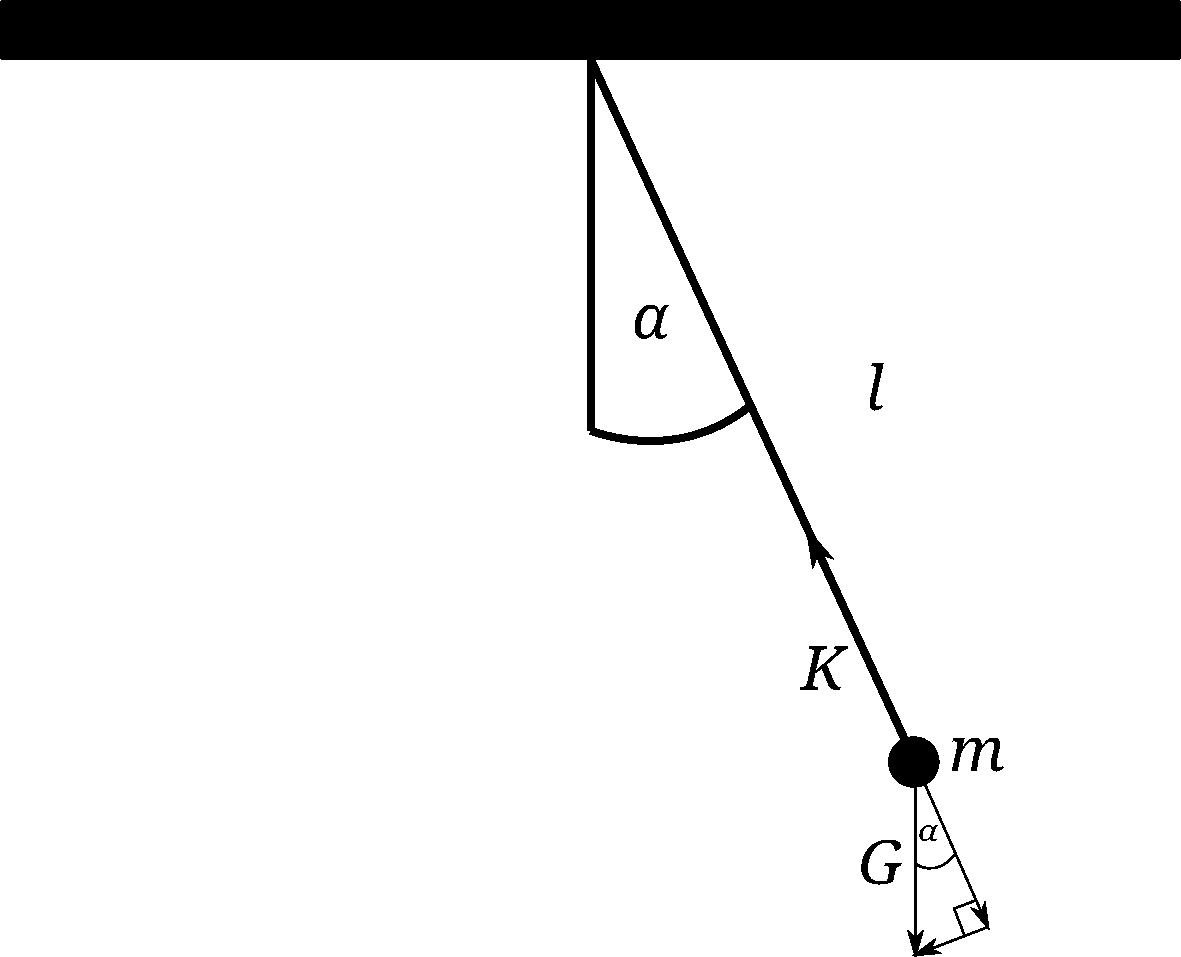
\includegraphics[width=\linewidth]{images/pendulum.pdf}
	\end{center}
	Az inga végén található súlyra felírva az érintő és sugár
	irányú erőket a következőt kapjuk:\\
	(1) $K - mg\cos\alpha = F_{cp} = ma_{cp} = m\frac{v^2}{l}$ \\
	(2) $-mg\sin\alpha = ma_{t}$ \\
	Ahol $K$ a kötélerő, $m$ a felfüggesztett test tömege, $g$ a
	nehézségi gyorsulás, $a_{cp}$ a centripetális gyorsulás, $a_{t}$ a
	tangenciális gyorsulás és végül $v$ a test sebessége. A (2)-es
	egyenlet negatív előjelét az indokolja, hogy az erő mindig a kitérés
	csökkenéséhez járul hozzá. \\
	A periódusidő meghatározásához nekünk a (2) egyenletre van szükségünk,
	hiszen az határozza meg a test pozícióját, míg az (1)-es egyenlet a
	geometriai viselkedését biztosítja. Átrendezve a következőt kapjuk: \\
	(3) $a_{t} = \beta l$ \\
	(2+3) $\beta = -\frac{g}{l}\sin\alpha$ \\
	Ahol $\beta$ a szöggyorsulás. Ez alapján nem tudjuk alkalmazni a
	harmonikus rezgőmozgáshoz ismert képletet, mivel a szög második
	deriváltja a szög szinuszától függ. Mivel tanulmányaim nem terjednek
	ki addig, hogy ezt a differenciál egyenletet megoldjam, ezért más
	módszert alkalmaztam.

\section{Numerikus analízis - \\ Euler algoritmus}
	Az Euler módszer kis szélességű téglányi területekkel közelíti
	meg a függvények alatti területet, amivel a számunkra szükséges
	szögpozíciót is megkaphatjuk. Az algoritmus a következő: \\
	$f''_{i} = $[állapot alapján kiértékelhető] \\
	$f'_{i} = f'_{i-1} + f''_{i}\Delta x$ \\
	$f_{i} = f_{i-1} + f'_{i}\Delta x$ \\
	Ahol $\Delta x \ll 1$. \\
	\\
	Ezt alkalmazva a problémára: \\
	$\alpha''_{i} = \beta_{i} = -\frac{g}{l}\sin\alpha_{i-1}$ \\
	$\alpha'_{i} = \omega_{i} = \omega_{i-1} + \beta_{i}\Delta t$ \\
	$\alpha_{i} = \alpha_{i-1} + \omega_{i}\Delta t$ \\
	A periódusidőt megkaphatjuk, ha megkeressük azt a $t \neq 0$
	időpillanatot, ahol a kitérés megegyezik a $t=0 $ időpontban
	lévővel.

\section{Százalékos eltérés}
	Az alább megadott paraméterek szerint készült a lentebb található grafikon,
	amely megmutatja az egyszerű fonálinga periódusidejéhez képesti százalékos
	eltérést minden fokra $\in (0,90] \cap \mathbb{Z} $: \\
	$l = 1m$ \\
	$g = 9.8\frac{m}{s^2}$ \\
	$\Delta t = 0.0001s = 100\mu s$ \\
	$T_{\alpha \ll 1} = 2\pi\sqrt{\frac{l}{g}}$ \\
	Az eredményekből láthatjuk, hogy kis szögekre $\alpha \ll 1$ vonatkozó képletet
	közel pontos eredményt ad. A grafikon más paraméterekre is ugyanazt az eredményt
	produkálja, így arra következtethetünk, hogy független azoktól.

\section{Hibahatár}
	Mivel a százalékos eltérés monoton, ezért egy adott százalékhoz tartozó
	fok megkereséséhez használhatunk bináris keresést. \\
	Az algoritmus lényege a
	következő: kijelölünk 2 pontot, az egyik határon belül lévő, a másik
	határon kívül lévő. \\
	Egy lépésben kijelölünk egy harmadik pontot, ami pontosan a
	kettő átlagán helyezkedik el. Ezután megvizsgáljuk, hogy ez a határon belül vagy
	kívül van, majd eszerint az elsőnek felvett 2 pont közül a megfelelő értékét
	átírjuk a 3. pontnak az értékére. Ezt egészen addig csináljuk amíg a 2 pont közötti
	távolság nem lesz $\leq\Delta\deg$. \\
	Mivel a futásidő $\mathcal{O}(\log_{2}n)$, így rövid időn belül, nagy pontossággal
	megkaphatjuk az értéket.\\
	Példának okáért 2\%-os hibahatáron belül maradáshoz a kapott érték:\\
	$\Delta\deg=0.000001\deg$ \\
	$\Delta t=0.00001s=10\mu s$ \\
	$\alpha = 32.1207920678108669817447500850574006528569...\deg$ \\
	Azonban figyelembe kell venni a periódus-számító algoritmus pontosságát a megadott
	$\Delta t$-vel, illetve a float szabvány limitációit, így az eredményt érdemesebb az
	alábbi közelítéssel megadni: $\alpha \approx 32.1 \deg$

\end{multicols}

\begin{center}
	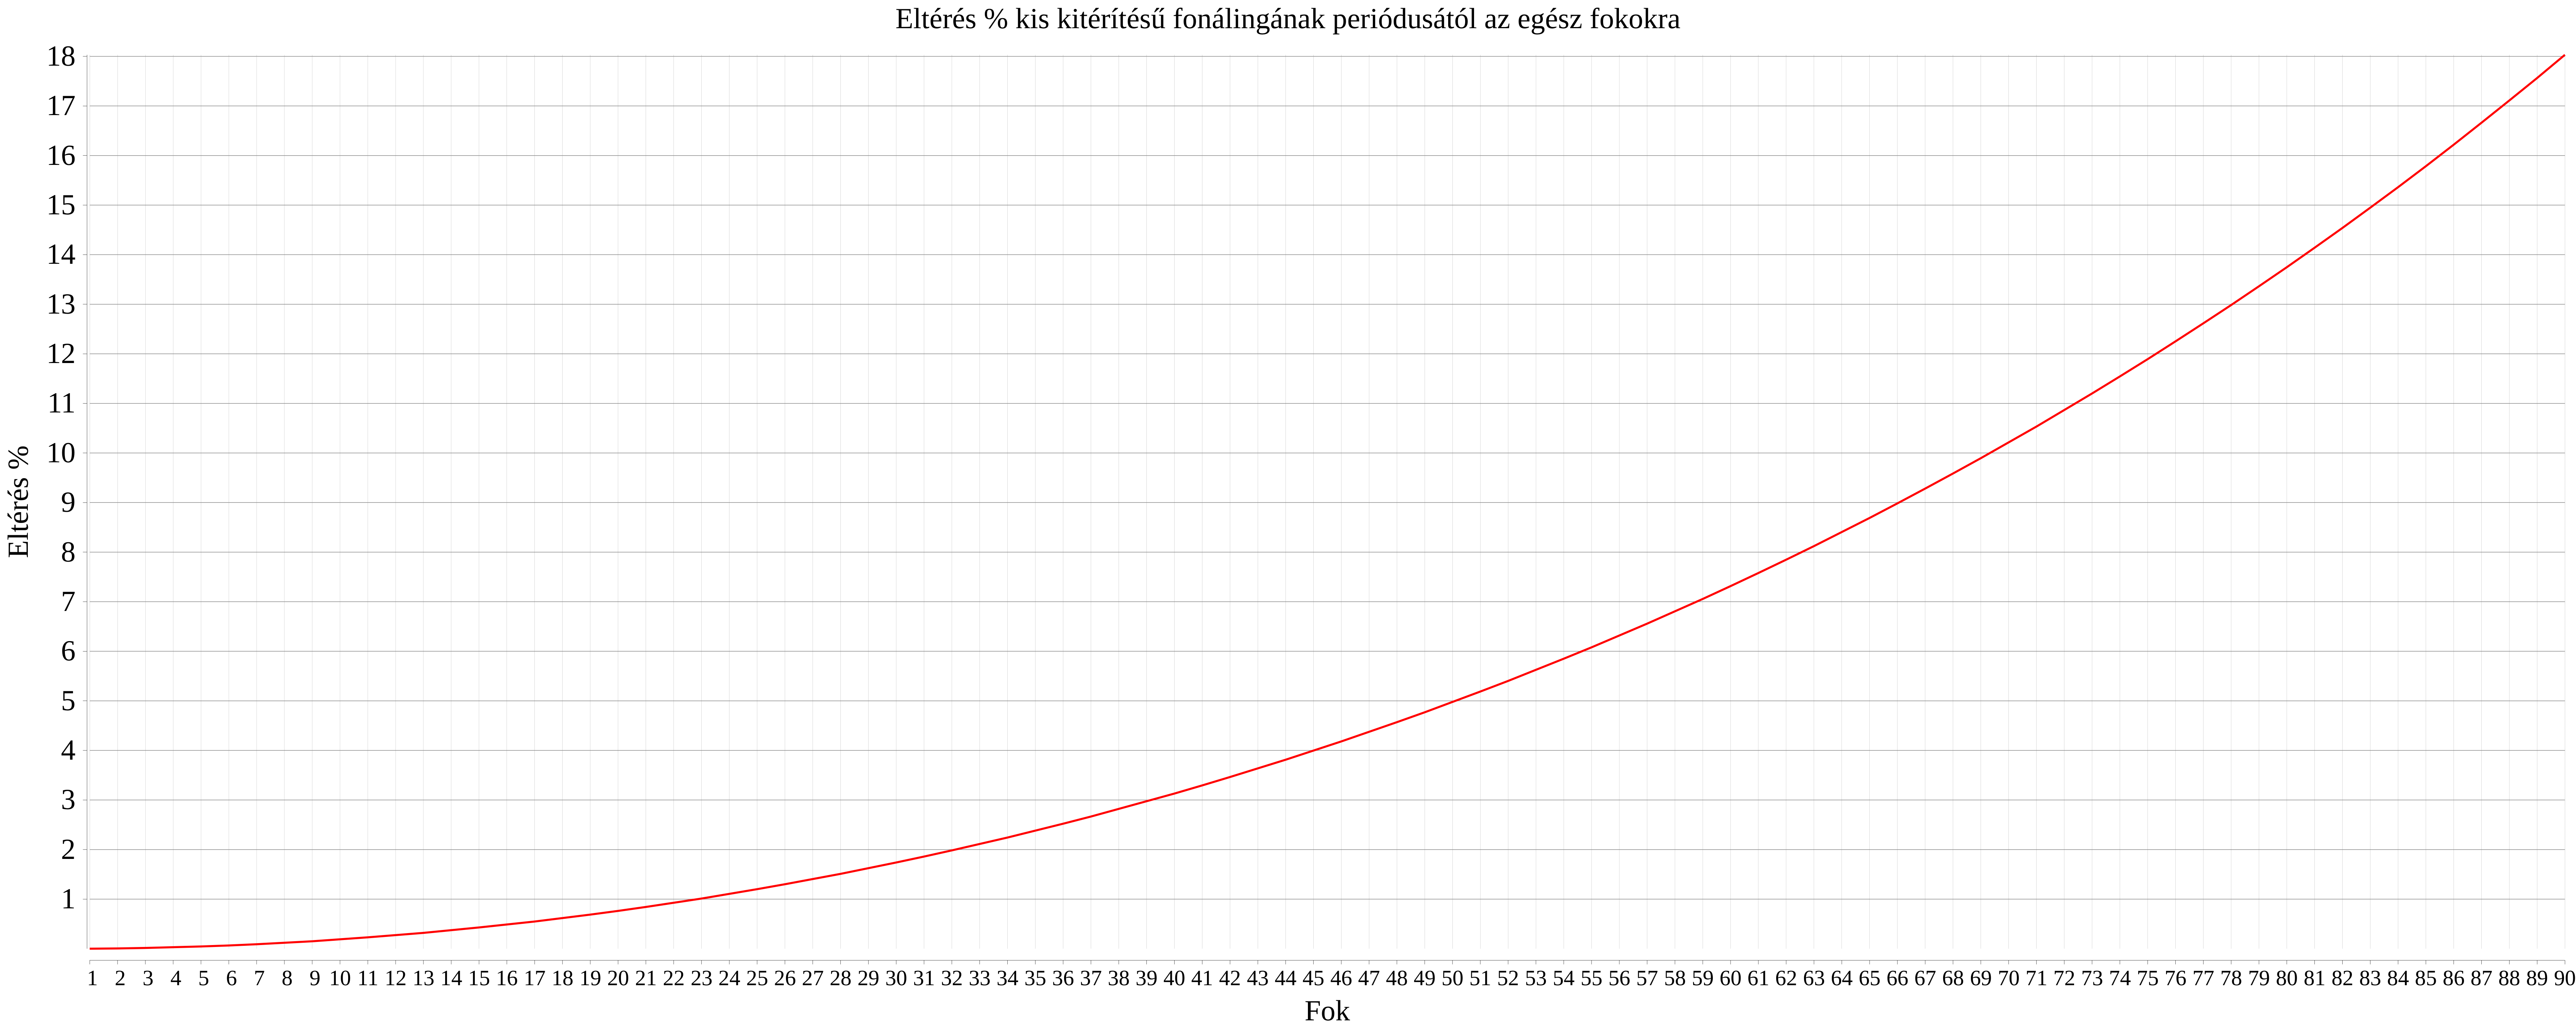
\includegraphics[width=\linewidth]{../difference.png} \\
\end{center}

\section{Kód - Lényegi rész}
	\lstinputlisting{../main.go}
\end{document}